\documentclass[preprint,12pt,authoryear]{elsarticle}
\usepackage{amsmath,amssymb,booktabs,tabularx,array,graphicx}
\usepackage[dvipsnames]{xcolor}
\usepackage[hypertexnames=false,colorlinks=true,linkcolor=MidnightBlue,citecolor=MidnightBlue,urlcolor=MidnightBlue]{hyperref}
\emergencystretch=3em
\journal{Computers \& Operations Research}
\newcommand{\TE}{\operatorname{TE}}
\newcommand{\ind}{\mathbf{1}}
\newcommand{\R}{\mathbb{R}}
\newcolumntype{Y}{>{\raggedright\arraybackslash}X}
\newtheorem{proposition}{Proposition}
\newproof{proof}{Proof}
\begin{document}
\begin{frontmatter}
\title{Ranked Execution: Cash-Funded Search for Sparse Portfolio Rebalancing}
\author{Artur Sepp}
\begin{abstract}
Implementing a target portfolio requires selecting and sizing trades under
funding, exposure and minimum-trade constraints. Ranked Execution combines
cash-funded marginal priorities, joint convex sizing and bounded search over
executable states, including screened trade replacements and restarts from
audited alternatives.
Mandatory interventions count towards the trade limit; only portfolios passing
an original-unit audit can replace the retained incumbent. A matched
mixed-integer formulation supplies reference solutions under identical inputs
and acceptance rules, with independent and heuristic-started calls reported
separately. A portable 302-ETF benchmark supplies 219 monthly decisions with
opaque identifiers. Ranked matches heuristic-started MIQP within $10^{-4}$ annual
basis points on all decisions, but the ticket allowance is nonbinding. A
frozen 24-case synthetic grid compares separate common-base and heuristic-started
joint MIQP calls at 10, 60 and 600 seconds. After correcting the reference's
numerical scaling and internal feasibility setting, Ranked ties all 24 independent
deliveries within the same band at every allowance. Independent MIQP is faster
at the median; additional time changes no delivered solution above the band.
No reported native bound contradicts an audited witness at the unchanged
comparison tolerance. All 182 synthetic arm outputs, including two tiny
controls, pass the original audit. Independent enumeration and conservative
relaxation bounds supply separate numerical controls. Neither conditional
comparisons nor retained-incumbent ties establish global optimality or realised
investment performance.
\end{abstract}
\begin{keyword}
portfolio rebalancing \sep trade cardinality \sep minimum trade \sep
tracking error \sep mixed-integer quadratic optimization
\end{keyword}
\end{frontmatter}

\section{Introduction}
A model portfolio describes desired exposures. Implementing every change can
require many small orders, while selecting only the largest weight changes
can overlook their joint risk consequences. The implementation problem is
therefore a discrete choice of trades followed by a continuous choice of
sizes. Funding, group exposures, minimum trade sizes and minimum held
positions couple these choices.

We study a conditional execution problem. Current holdings, target weights,
a covariance estimate and execution constraints are supplied inputs. The
task is to reduce tracking variance to the target using a limited number of
actual noncash trades. A trade limit counts movements from the current book;
it is distinct from a limit on terminal holdings. Cash is the settlement
coordinate and need not be riskless. Required interventions, such as an exit
or an upper-bound correction, consume tickets even when explicitly exempted
from a minimum order size.

Ranked Execution evaluates cash-funded marginal directions and then jointly
sizes selected executable states. Single-name improvements are supplemented
by a bounded shortlist of coordinated state changes. These can admit a
funding pair whose isolated trades are unhelpful, or expose another
instrument after an earlier useful pair. Every accepted improvement passes
the same original-unit audit. A native solver status alone does not establish
portfolio acceptance.

The contribution has three parts. First, the formulation keeps original
holdings, a prepared feasible base and raw model targets distinct. This
separation makes mandatory accounting and minimum-ticket semantics explicit.
Second, the search combines inexpensive covariance-aware priorities with
joint sizing under the complete coupled constraints. Third, a portable
benchmark and independent checks expose failures, search limits, timing
and dependence on supplied incumbents.

The empirical input universe comprises 302 publicly traded ETFs. Model
weights and covariances are frozen before execution comparisons. Numerical
instances have opaque asset identifiers and contain no private fund
observations. Readers do not need proprietary signals or a risk-model
refit to reproduce execution. Each decision begins from the drifted previous
model allocation, so every method receives identical current holdings.
This experiment measures conditional implementation decisions, not
strategies recursively evolving their own holdings.

A full joint mixed-integer reference fixes the objective, admissible states and
return audit. A separate call receives the heuristic's incumbent and charges
its generation time explicitly. Three time allowances distinguish additional
search opportunity from the effect of that start. Development ablations remain
in the replication archive. The separate operational MIQP policy has different
objective and constraint options and is outside this matched comparison.

\section{Related work}
Cardinality-constrained portfolio selection and index tracking have a
substantial optimization literature. \citet{mutunge2018} analyse covariance
tracking with a restricted number of holdings and study greedy construction
and exchange improvement. This is a close methodological reference.
Here cardinality applies to movements from an existing portfolio, with a
distinguished funding coordinate and executable trade/holding intervals.

Restricted-support search is also established. \citet{kernel2012} develop
Kernel Search for mixed-integer index-tracking formulations by exploring
restricted portions of the feasible region. Ranked Execution shares the
principle of prioritising small subproblems. Its priority comes from
one- and two-coordinate cash-funded quadratics; the subsequent subproblem
sizes the entire selected support under coupled constraints.

\citet{strub2018} formulate an index-tracking rebalancing problem that
explicitly balances transaction costs and tracking accuracy. Our objective
is ex-ante tracking variance with hard operating rules. Transaction-cost
minimisation, market impact and execution scheduling are outside the model.
A ticket cap is an operating constraint, not a calibrated replacement for
every source of trading cost.

\citet{bertsimas2022} develop scalable outer approximation for sparse
portfolio selection using ridge regularisation and a convex binary
reformulation. This demonstrates the value of strong formulations and
carefully designed computation. We do not claim that bounded local search
supersedes those methods. Greedy selection, convex sizing and support
exchange are established ideas; the present contribution combines them
with conditional trade states, funding and audited delivery.

The empirical question is how well this specific combination approximates
a matched mixed-integer solution under declared computational controls.
Direct comparisons with additional established methods on the same trade
domain remain an extension. Differences in objectives and constraints
must be resolved before algorithms from other portfolio formulations can
serve as matched controls.

\section{Conditional execution problem}\label{sec:problem}
\subsection{Inputs and objective}
Let $c,m,w\in\R^N$ denote current, model and delivered weights, measured as
fractions of net asset value. Index $k$ identifies settlement cash and
$\Sigma\succeq0$ is the supplied annual covariance matrix. The objective and
reported tracking error are
\begin{equation}\label{eq:objective}
 f(w)=(w-m)^\top\Sigma(w-m),\qquad \TE(w)=\sqrt{f(w)}.
\end{equation}
Annual basis points equal $10^4\TE(w)$. No alpha term, turnover penalty or
class-specific risk price enters this execution objective.

The long-only hard domain includes
\begin{equation}\label{eq:linear}
 \mathbf{1}^\top w=1,\quad L\le w\le U,\quad a\le Aw\le b.
\end{equation}
Group rows may be fractional: a mixed-asset instrument need not belong
wholly to one group. Bounds and eligibility can encode calendar restrictions
and instructions. Cash bounds are real constraints; funding through cash
does not imply unlimited borrowing or unrestricted cash deployment.

A terminal noncash holding is zero or at least its declared floor:
\begin{equation}\label{eq:floor}
 w_i=0\quad\text{or}\quad w_i\ge\theta_i,\qquad i\ne k.
\end{equation}
An ordinary discretionary movement satisfies
\begin{equation}\label{eq:ticket}
 w_i=c_i\quad\text{or}\quad |w_i-c_i|\ge\delta_i.
\end{equation}
The minimum applies to the delivered order, not merely to the desired
model-current difference. Joint sizing can otherwise reduce an eligible
desired trade to a much smaller actual movement.

Let $\tau_i(w)=\ind\{w_i\ne c_i\}$ be the mathematical trade indicator.
The total noncash count satisfies
\begin{equation}\label{eq:cap}
 \sum_{i\ne k}\tau_i(w)\le K.
\end{equation}
Numerical delivery uses a separately declared trade-zero threshold.
The model does not impose a terminal position-count limit.

\subsection{Mandatory declarations and corridors}
The consumer resolves lifecycle transitions, instructions and ordinary
product bounds before risk search. Let $q^0$ be the resulting funded base.
Every noncash base-current movement receives a mandatory category.
A required correction can have a fixed endpoint or a one-sided interval
allowing further movement in the permitted direction. A minimum-ticket
exemption removes only the minimum-size condition: it does not remove the
trade from the count or waive a holding floor.

For optional instrument $i$, an ordinary corridor lies between its base and
target, intersected with eligible hard bounds:
\begin{equation}\label{eq:corridor}
 [\ell_i,h_i]=[\min(q_i^0,m_i),\max(q_i^0,m_i)]\cap[L_i,U_i].
\end{equation}
The actual supplied intervals also retain lifecycle decisions, pins and
declared preparation exceptions. Mandatory instruments keep their own
resolved intervals. Cash retains its hard funding interval instead of a
model-current corridor.

Before solving, declarations must be reconciled with compiled rows. Each
enabled group requires an unambiguous label, a finite membership vector
and its original lower and upper limits. A missing membership column is an
input error, not a zero vector. An intentionally empty group is redundant
only if $a_j\le0\le b_j$; emptiness must be explicitly acknowledged. A
positive lower bound on an empty group is contradictory. Reconciliation
records the source declaration, compiled identifier, coefficients and
bounds, including distinct identifiers for homonymous groups. The final
exposure and residual are reported against those rows. This pre-solve
check closes a gap that a return audit alone cannot detect: an omitted
constraint is absent from the audit as well. Reconciliation changes no
objective coefficient, endpoint or numerical tolerance.

The eligible hard domain permits movement within full resolved product and
instruction bounds. We call the two domains CORRIDOR and FULL. They answer
different optimization questions. Every algorithm in the main comparison
uses CORRIDOR. FULL is used by common preparation only when the ordinary
corridor cannot supply a valid base.

If the policy declares a discretionary allowance $B$, the total cap is
$K=M+B$, with $M$ unique active mandatory names after preparation. This is an
explicit convention. An input declaring a fixed total cap must retain it;
preparation cannot silently enlarge that cap when declaring another repair.

\subsection{Common feasibility preparation}
Individual lifecycle decisions can produce a base that violates funding,
group bands or holding floors. Separately repairing each algorithm's
base would conflate preparation and risk-search effects. We prepare one
shared instance before running any comparison arm.

An already audited base is retained exactly. Otherwise, preparation searches
CORRIDOR and then, if needed, eligible FULL bounds. Its objectives are
risk-neutral. In FULL, corridor excursion is minimised before gross noncash
intervention and the number of additional repair instruments. Within the
selected discrete pattern, a strictly convex squared-intervention objective
breaks continuous ties. Target risk and alpha do not choose among repairs.

Additional noncash interventions are pinned, declared and counted before
risk search. Endpoints outside an original corridor are recorded as
preparation exceptions, while full hard bounds and eligibility remain
unchanged. All arms receive the same final base $q$, intervals, mandatory
flags, exemptions and resolved cap.

Sequential optimization stages use an explicit numerical objective guard;
they are not exact symbolic lexicographic arithmetic. A shared 30-second
allowance includes preparation stages. Failed preparation remains in the
experiment denominator. A numerical failure or exhausted budget alone does
not establish mathematical infeasibility. Conditional solver comparisons
state how many inputs successfully prepared.

\section{Executable states and matched formulation}\label{sec:states}
\subsection{Finite unions of intervals}
For each noncash instrument $i$, compile a finite family of executable alternatives,
$\mathcal J_i=\{[\ell_{ij},h_{ij}]:j\in J_i\}$.
For an ordinary optional instrument these include the no-trade point when
valid, a sell interval ending at $c_i-\delta_i$, and a buy interval starting
at $c_i+\delta_i$. Intersect the alternatives with the permitted corridor and
with $\{0\}\cup[\theta_i,\infty)$, and remove empty intervals. Mandatory
exemptions and fixed pins are applied before compiling the states.

Each state carries a ticket flag $t_{ij}\in\{0,1\}$ measured from original
holdings. An optional no-trade point has flag zero; an exempt mandatory
movement keeps flag one. Once states are fixed, remaining sizing is a
continuous convex problem.

For example, let $c_i=0.02$, the corridor be $[0,0.04]$,
$\delta_i=0.005$ and $\theta_i=0.01$. The alternatives are a no-trade point
at $0.02$, a full exit at zero, a sell interval $[0.01,0.015]$, and a buy
interval $[0.025,0.04]$. Selecting a sale does not prescribe its unique size.
Funding and group constraints determine final size jointly with other names.
Several states never create several tickets for one instrument.

\subsection{Full joint MIQP reference}\label{sec:miqp}
Introduce binary selectors $z_{ij}\in\{0,1\}$ and continuous contributions
$v_{ij}$. The full joint model chooses every state and trade size together:
\begin{align}\label{eq:joint-miqp}
 \min_{w,v,z}\quad &(w-m)^\top\Sigma(w-m)\\
 \text{subject to}\quad
 \sum_{j\in J_i}z_{ij}&=1,&
 \ell_{ij}z_{ij}\le v_{ij}&\le h_{ij}z_{ij},\\
 w_i&=\sum_{j\in J_i}v_{ij},&
 \sum_{i\ne k}\sum_{j\in J_i}t_{ij}z_{ij}&\le K.
\end{align}
and all funding, instrument and group rows in \eqref{eq:linear}. This is a
convex mixed-integer quadratic problem (MIQP). A declared optional allowance
adds its corresponding sum over optional names. Cash has no trade selector.

Every method uses the same prepared state domain. ``Full joint'' means all
choices are optimised together; it does not mean replacing the prepared
CORRIDOR domain with the wider FULL preparation domain. The model's optimum
cannot be worse than a feasible heuristic vector in this domain. The historical
replication identifier \texttt{Exact} names the formulation, not a certificate
for every returned vector. The implementation solves an equivalent
conic canonical representation. Native status, native incumbents and
externally retained weights remain separately attributed.

The operational \texttt{execution/MIQP} implementation is a separate policy:
it permits an alpha trade-off, a terminal position cap and repair-on-touch
rules. Those options are absent from this tracking-variance benchmark.
Its outputs would confound policy and algorithm effects, so they are not
included as an additional matched arm.

Fixing one state per instrument yields a convex quadratic program. Fixed
coordinates and cash can be eliminated algebraically. Heuristic supports use
the same joint-sizing formulation. A conditional fixed-state refinement of
an integer incumbent preserves its declared state choices and is audited
separately; native outputs are never rounded into acceptance.

\section{Ranked Execution}\label{sec:algorithm}
\subsection{Cash-funded marginal gains}
A change in noncash instrument $i$ is funded through $u_i=e_i-e_k$.
At working point $w$, define
\begin{equation}
 g_i=u_i^\top\Sigma(w-m),\qquad s_i=u_i^\top\Sigma u_i\ge0.
\end{equation}
A displacement $x$ changes risk by
\begin{equation}\label{eq:gain}
 f(w+xu_i)-f(w)=2g_i x+s_i x^2.
\end{equation}
For state displacement interval $D_i=[d_i^-,d_i^+]$, minimise this scalar
quadratic. When $s_i>0$, the minimiser is the projection of $-g_i/s_i$
onto $D_i$; when $s_i=0$, an endpoint minimises the linear expression.
Ties are resolved deterministically.

The priority is the negative objective change at that minimiser. Greedy
selection admits positive-gain optional names within the allowance and
updates covariance products after each virtual move:
\begin{equation}
 \Sigma(w-m)\leftarrow\Sigma(w-m)+x_i(\Sigma_{:i}-\Sigma_{:k}).
\end{equation}
A selected name cannot consume another ticket by choosing a second state.
Instrument identifiers and state indices break score ties.

Virtual working points are support proposals. They need not satisfy
coupled cash or group bounds. Those constraints enter joint sizing, and only
an audited jointly sized vector can replace the incumbent. A marginal
priority guides computation without becoming an acceptance rule.

\subsection{Joint sizing and mandatory coordinates}
The search starts from the shared audited incumbent $q$. A mandatory-only
QP first explores movable mandatory coordinates and their bounded holding
alternatives. A feasible base can still be improved along these coordinates;
an empty optional support must not suppress their optimization.

For a proposed optional support, selected states are free within their
intervals; unselected optionals remain at base. Movable mandatory
coordinates and cash are jointly sized with them. Funding, instrument
bounds and original group rows are included. Every candidate is audited
before retention.

The default explores at most 32 mandatory state combinations per support.
Truncation is reported. Failure of one assignment does not prove that every
assignment for those instrument names is infeasible. A feasible candidate
with more risk than the incumbent leaves the incumbent unchanged.

If initial greedy sizing supplies no audited candidate, a bounded rescue
list tries constraint-directed admissions, removals and replacements.
Its separate allowance is at most 24 support trials. Rescue respects the
same cap and states; it cannot introduce a new exemption or broaden a
corridor.

\subsection{Coordinated state changes}
Isolated priorities can miss a useful combination. Funding and group
restrictions may make a buy and sale jointly attractive even when their
isolated proposals are unsuitable. The method supplements one drop and one
exchange pass with a bounded coordinated neighbourhood.

At incumbent $\bar w$, let $C_{ij}=u_i^\top\Sigma u_j$. For proposed
state-displacement intervals $D_i,D_j$, the two-coordinate priority is
\begin{equation}\label{eq:pair}
 -\min_{x\in D_i,\,y\in D_j}
 \{2g_i x+2g_j y+C_{ii}x^2+2C_{ij}xy+C_{jj}y^2\}.
\end{equation}
The positive-semidefinite box quadratic is evaluated through boundary minima
and any admissible interior stationary point. This priority is inexpensive
relative to complete joint sizing.

The neighbourhood changes one or two optional states: admissions, removals,
replacements within available slots, or holding alternatives. Priorities do
not include all coupled rows or reoptimisation of the other selected
coordinates. Consequently, even a negative isolated priority need not
exclude a support from the shortlist.

The best unvisited candidates form a bounded shortlist. Joint sizing evaluates
them under all constraints. If the incumbent improves and trials remain,
the search restarts from the new incumbent. At most three anchors share a
total coordinated budget of 24 support trials. A pass without improvement
stops the stage. These are support trials; mandatory alternatives and
numerical retries can require more than 24 native QP calls.

\subsection{Scarce-ticket extension}
When the optional candidate count exceeds a positive allowance, the completed
search above is retained and a separate branch explores scarce-ticket combinations.
First, solve the continuous perspective model of the same state formulation.
In funded coordinates $w=r+Ux$, write $H=U^\top\Sigma U$ and choose
$D=\operatorname{diag}(d)$ with $d\ge0$ and $H-D\succeq0$.
The implementation uses half the nonnegative minimum eigenvalue of the
diagonally normalised active block of $H$, multiplied by its diagonal,
and verifies the residual matrix. Retain the constant and affine terms of
$f(r+Ux)$ and replace its quadratic part by
\[
 x^\top(H-D)x+\sum_i d_i x_i^2/z_i,
\]
where $z_i$ is the sum of optional ticket-state selectors and equals one
for mandatory coordinates. The closed perspective uses zero at $(x_i,z_i)=(0,0)$
and excludes $x_i\ne0$ when $z_i=0$. Relax selectors to their continuous hull
only for this guidance solve. At executable integer states the objective is
the original quadratic; the integer reference remains the matched formulation above.
Rank optional names by fractional ticket occupancy, choose each name's highest
occupancy ticket state, and round the first $B$ names into a support. Identifiers
and state indices resolve ties. Fractional weights are never returned: the rounded
support must pass the unchanged joint-sizing QP and original-unit audit.
An audited seed may initially be inferior; its search branch is kept separate
and the original incumbent is restored unless the completed branch strictly improves it.

At each scarcity anchor, jointly size every one-for-one optional replacement.
This sweep allows all retained coordinates to resize. Merely scoring the removed
and admitted coordinates can miss an improvement that requires that recourse.
The expanded neighbourhood also admits two new names coupled to one or two
removals, making a two-for-two replacement reachable at a full ticket budget.
Its two-coordinate priority includes cash and group rows through polygon clipping
and quadratic minimisation on edges and the interior. If that fixed-coordinate
slice is empty, retain the box priority in \eqref{eq:pair}: other selected names
can move during joint sizing, so an empty slice is not a support infeasibility proof.
For a coupled removal, include its exact cash-funded quadratic change in the score.

The rounded seed and expanded shortlist share a separate 24-support allowance.
Up to three anchors each have a complete single-replacement sweep; these sweeps
are additional work, not part of the 24-support count. After a shortlisted
improvement, restart early when another anchor is available. Stop after an
unimproved pass. Search is bounded but neither local nor global optimality follows.
The extension uses no integer solve and no reference-arm incumbent. Its continuous
model supplies priorities only; it does not change the delivered objective,
constraints, mandatory declarations or acceptance tolerances.

The final pair replacement can expose a useful single replacement after the last
sweep. Also, an inferior or infeasible rounded seed can lead to a better support
through joint resizing. We therefore run a final replacement branch from the
completed incumbent and from the unrestricted rounded seed. To diversify beyond
pair replacements, pin one selected name at its no-ticket state in a temporary
continuous guidance model, round the resulting occupancies and search that seed.
At most $\min(B,24)$ incumbent names are tried, in identifier order; duplicate
seeds are skipped. The pin affects guidance only: every candidate is sized and
audited on the original problem, and the excluded name may re-enter a branch.

Each distinct seed receives at most three complete single-replacement sweeps.
If its initial sizing fails, the first sweep still tries replacements around
the proposed support. Subsequent sweeps use the best audited branch support and
stop without improvement. Each branch is compared to the separately retained
completed incumbent. A per-call cache stores the best audited original-domain
sizing result, or failure, for each support over the same bounded mandatory
assignments. Separate branch visitation allows a cached support to serve as an
intermediate point without another QP. This bounded diversification can cross
more than two replacements in total; it is not exhaustive multi-name enumeration.

An empty optional incumbent has no names to exclude. Moreover, a promising
combination can require retaining a particular trade, rather than removing one.
A further bounded phase therefore takes the union of the completed incumbent's
ticket states and the unrestricted rounded seed's ticket states. In stable
instrument/state order, it conditions on inclusion and then exclusion of each
state, stopping after at most 24 additional continuous solves. Inclusion fixes
that state selector to one; exclusion fixes it to zero. All other objective terms,
rows and numerical tolerances remain unchanged. The rounding step respects the
decision, prioritising a forced admission over unconstrained choices.

Each distinct proposal receives the same replacement restart, including rescue
around infeasible seeds. A final restart revisits the completed incumbent.
These temporary selector conditions guide proposals only: executable sizing uses
the original problem, and every branch competes with the retained audited
incumbent. This phase is a finite conditional neighbourhood, not recursive
branch-and-bound. Its continuous objective values are not optimality certificates.

\paragraph{Screened pair completion}
Slice priorities hold retained positions fixed, whereas joint sizing can resize
them. Consequently a low-priority pair can still improve the portfolio. An additional
phase shares at most $R^2$ additional coordinated trials across the same anchor
limit, where $R=24$ is the rescue allowance: 576 trials and at most three anchors
by default. Each anchor retains the complete single-replacement sweep. All
previously sized supports are skipped; strict audited improvements re-anchor
the search while passes remain. The earlier incumbent is always retained.

An inexpensive necessary-feasibility screen precedes the shortlist. Selected
coordinates and cash span their original intervals, unselected coordinates stay
at the base, and mandatory coordinates span the union envelope of their states.
For each funding or group row, interval arithmetic gives its smallest and largest
possible value, using the coefficient sign to select each endpoint. Existing
coordinate and row audit allowances yield a conservative outer envelope. A
support is rejected only if this envelope cannot intersect a required row interval.
Surviving supports still pass unchanged original-domain joint sizing and audit;
the screen neither relaxes an executable constraint nor proves joint feasibility.
It removes obvious dead ends without suppressing recourse in retained positions.
The finite trial and anchor budgets can still miss improving combinations.

\paragraph{Cached alternative restarts}
Improving-only descent can stop before a feasible three-position replacement.
The sizing cache already contains audited alternatives that were not retained.
Order these by objective and then instrument/state identifiers, exclude the
current support, and restart from at most $R$ alternatives. Each branch uses the
same bounded complete single-replacement sweeps and separately retains the
incumbent. A worse seed may therefore connect a useful sequence of supports.
At the first branch improving the incumbent, complete its pair neighbourhood
once using another $R^2$ trial allowance and the same anchor limit, then stop.
The support list is selected before these restarts; it uses no reference-arm
portfolio. Failed branches cannot worsen delivery. This finite search broadens
coverage without establishing exhaustive three-position optimality.

\begin{table}[!ht]\centering\small
\caption{Ranked Execution with audited incumbent retention.}
\begin{tabularx}{\linewidth}{rY}\toprule
Step & Operation\\\midrule
1 & Validate inputs, compile states and audit the shared prepared base.\\
2 & Size movable mandatory states without optional trades.\\
3 & Construct cash-funded greedy priorities and jointly size selected states.\\
4 & If needed, attempt the bounded feasibility-rescue shortlist.\\
5 & Attempt one drop and one exchange pass over the initial accepted support.\\
6 & Jointly size coordinated changes; restart after improvement while the shared
trial and anchor allowances permit.\\
7 & Under ticket scarcity, retain this incumbent; jointly size a perspective-guided
seed, complete single replacements and shortlisted pair replacements.\\
8 & Search final replacement sweeps and distinct seeds from temporarily excluded
incumbent names; size every candidate on the original problem.\\
9 & Include/exclude states from the incumbent and tentative relaxed seed in bounded
guidance calls; search distinct proposals and revisit the completed incumbent.\\
10 & Revisit the completed incumbent with the interval-screened pair allowance;
jointly size each shortlisted support on the original domain.\\
11 & Restart from bounded cached audited alternatives; after the first improving
branch, complete its pair neighbourhood once.\\
12 & Return the best audited branch, with all search work and failures recorded.\\
\bottomrule\end{tabularx}
\end{table}

\subsection{Properties and computational cost}
\begin{proposition}[Conditional incumbent retention]\leavevmode\par
For fixed arrays and acceptance rules, if the initial incumbent passes the
return audit and replacement requires an audited strict objective improvement,
the returned objective is no worse than that of the initial incumbent.
\end{proposition}
\begin{proof}
The initial incumbent is stored. Each replacement passes the same audit and
has smaller objective. Failure to find a replacement leaves it unchanged.
\end{proof}
This delivery property is equally available to the mixed-integer reference.
It is not an approximation ratio or an optimality certificate and says
nothing about future risk after rolling holdings diverge.

For dense covariance, the initial covariance-vector product costs $O(N^2)$.
With bounded states per instrument, each greedy score and column update
costs $O(N)$, giving $O(N^2+BN)$ arithmetic for that stage and $O(N^2)$ input
storage. These counts exclude validation, convex sizing, mandatory
enumeration and improvement search.

With $s$ available state changes, coordinated enumeration can inspect
$O(s^2)$ pairs per anchor. A bounded shortlist does not make its generation
constant work in universe size. Support-key construction and ordering add
overhead. The scarcity extension can enumerate $O(B^2s^2)$ pair replacements
per anchor, plus at most $Bs$ jointly sized single replacements. It also solves
one unrestricted and up to $\min(B,24)$ restricted continuous perspective problems.
The final incumbent, unrestricted seed and distinct restricted seeds add at most
$2+\min(B,24)$ branches, each with at most three sweeps of $Bs$ supports.
If the conditional phase considers $C\le24$ decisions, it adds $C$ continuous
solves and at most $C+1$ replacement branches. Each branch sizes its seed and
at most three sweeps of $Bs$ supports. Caching removes duplicate sizing work
within a call. Each earlier stage has
at most three anchors and its own shortlist allowance; mandatory enumeration
multiplies sizing counts.
The screened completion phase adds at most $R^2$ coordinated supports and three
single-replacement sweeps. Its interval screen costs $O(mn)$ per candidate for
$m$ group rows and $n$ instruments, in addition to pair-priority generation.
Cached alternatives add at most $R$ branches of three $Bs$ replacement sweeps.
The first improving branch permits at most one further completion phase with
the same bounds. Cached results avoid duplicate QPs, but scoring and revisiting
supports still incur work.
These additional costs are measured rather than hidden inside the initial
greedy complexity. A support cap is not a wall-clock guarantee.

The library accepts exact factor-plus-diagonal covariance representations
when available. The empirical comparison retains its supplied dense
matrices, including residual correlations. Substituting a diagonal residual
approximation would change the experiment and is not done here.

\section{Numerical acceptance and comparison protocol}\label{sec:audit}
\subsection{Original-unit audit}
Every final vector is checked in NAV fractions against unchanged supplied
arrays. Feasibility tolerance is $10^{-7}$ and actual-trade zero is $10^{-8}$.
Holding floors and minimum tickets retain their declared values. The
independent benchmark audit checks funding, instrument intervals, group
exposures, floors, nonexempt ticket sizes and both ticket allowances. It calls
neither the implementation's state compiler nor its audit evaluator.
Returned vectors are not renormalised or rounded.

Numerical QPs express movable weights in basis points, eliminating fixed
coordinates and cash algebraically. In fixed-state sizing, a bound or group
row is removed only when every remaining variable coefficient is exactly
zero and its constant value satisfies both unchanged endpoints.
Nonzero coefficients, however small, and constant contradictions are retained.
This algebraic reduction avoids degenerate constant rows without enlarging
the feasible set. Integer hulls retain every linear row; their quadratic cone
is balanced as described below. Continuous relaxation graphs are unchanged.
Group rows use the same bounded residual
envelope as the original-unit audit. Original limits remain authoritative at
return. CLARABEL uses absolute/relative gap and feasibility controls of
$10^{-10}$. A numerical solver exception permits one fresh attempt with
equilibration disabled, retaining the graph, objective, rows and tolerances.
An infeasible status does not trigger that retry.

The qualified implementation reuses compiled sizing graphs only when canonical
sparse coefficients agree exactly with a fresh construction. Each trial still
receives a fresh numerical solve and the same audit; no trials or constraints
are dropped. A failed equivalence check uses the ordinary construction. This
reduces compilation overhead without changing the search or measured weights.

This aligns numerical construction and acceptance. It does not prove literal
feasibility beyond the declared tolerance, or convert a native lower bound
into a certified optimality gap. The benchmark records raw statuses and
candidate rejection alongside delivered portfolios.

\subsection{Three principal comparisons}
Table~\ref{tab:arms} specifies the principal comparisons. Common preparation is
performed once and fixed across arms. Common-base MIQP starts from the prepared
incumbent. V2-started MIQP is a separate call supplied with Ranked's incumbent.
Neither call receives a pooled best result across algorithms.

\begin{table}[htbp]\centering\small
\caption{Arms under the same prepared CORRIDOR domain.}\label{tab:arms}
\begin{tabularx}{\linewidth}{lY}\toprule
Arm & Definition\\\midrule
Ranked (V2) & Full default search, including all scarcity extensions;
up to three anchors per stage and separately recorded sweeps.\\
MIP-B & Full joint model started from the prepared base (\texttt{ExactBase}).\\
MIP-V & Separate full joint solve started from V2 (\texttt{ExactRanked}).\\
\bottomrule\end{tabularx}
\end{table}

The ETF comparison uses a 10-second wrapper allowance; the synthetic study
uses separately started 10/60/600-second calls. All use one native thread, seed
zero and relative MIP-gap setting $10^{-4}$. Graph construction, start
lifting and conditional fixed-state refinement consume this allowance.
Native operations can overrun it; measured wall times are reported.

An earlier native integer feasibility setting of $10^{-4}$ produced a false
optimal termination on the overlapping-group instance \texttt{joint\_007}.
The native lift of a better feasible portfolio reproduced its objective, and
an independently formulated full-weight fixed-support QP confirmed the witness.
Tightening only native integer feasibility to $10^{-9}$ recovered the better
solution without supplying it as a start. Disabling presolve also recovered it;
additional time alone did not. Tightening that setting alone left smaller
bound inconsistencies. For integer hulls we therefore also replace
$x^\top Qx/10^4$ by $(x/100)^\top Q(x/100)$ in the conic graph, where $x$
is funded displacement in basis points. This balances the quadratic epigraph
without changing its value, any linear row or the native start mapping.
Fixed-state sizing and continuous relaxation graphs are unchanged.
The correction changes internal numerical
accuracy, not the objective, state constraints, original-unit audit or other
solver tolerances. The ETF and full joint tables use both corrections; earlier
search-development records retain their original source hashes.

Raw native statuses and bounds remain visible. A consistency check compares a
native bound with the delivered incumbent, and the benchmark separately checks
it against every audited cross-arm witness at the existing $10^{-12}$ variance
comparison scale. Bounds are never clipped to an incumbent. Passing these
checks is not an independent global certificate.

The ETF replication also retains Greedy (without support rescue or improvement)
and OneAnchor (one coordinated anchor per stage and one replacement sweep per
diversification branch). Their results and the earlier search-development
studies remain available as ablations rather than additional headline methods.

Native audited incumbents, retained external starts and refined candidates
have distinct attribution. An ExactRanked delivery equal to Ranked does
not establish independent native discovery. An ExactBase delivery worse
than Ranked under a time limit does not mean its mathematical optimum is worse.

Arms run serially on one host. Algorithm-call times exclude imports and
input loading. Preparation is reported separately and included in
end-to-end time. ExactRanked additionally includes its Ranked start-generation
cost. These are declared computational controls, not equal elapsed budgets.
The recorded host runs Windows 11 on an Intel Core Ultra 7 265 processor.
The rerun uses Python 3.12.14, unreleased corrected OP source with 9.1.5
metadata, QIS 5.44.4, CVXPY 1.9.2, MOSEK 11.2.3 and CLARABEL 0.11.1.
The public PyPI 9.1.5 wheel does not contain this correction; accompanying
source hashes identify the implementation. The replication protocol records the full
numerical package versions and execution-source hashes.

An earlier archived ETF run used a different preparation implementation and
dependency cohort; its allocation changes cannot be attributed to this search
extension alone. A separate regression control repeats all 219 decisions with
published OP 9.1.5 under the current dependencies. Its Ranked weights and TE
values are exactly identical to the corrected source on every decision.
The scarce-ticket extension is inactive in these cases. Control timings are
excluded because verification ran concurrently; the five-arm timings below
come from the serial primary run.

\section{The 302-ETF benchmark}\label{sec:benchmark}
\subsection{Frozen supplied inputs}
The source universe contains 302 publicly traded ETFs, retrospectively
selected in October 2026. Frozen model allocations span June 2008 through
September 2026. We construct 219 monthly decisions from July 2008 onward.
Eligible covariance support expands with available observations. The supplied
universe is not a point-in-time investable-universe reconstruction.

Each case begins from the previous supplied model portfolio, normalised once
to unit investment and drifted through the intervening month with the
canonical portfolio helper. This removes the previous model's small
investment residual when defining the hypothetical current book.
The current raw target remains unchanged in the risk objective.
No competing execution strategy's historical holdings define these cases.

The experiment is conditional on supplied targets and risk estimates.
It does not validate upstream model selection, estimate the economic value
of signals or establish out-of-sample investment performance. Monthly cases
share assets and market history and are not treated as independent samples.

Every instrument has a 10\% upper bound, including settlement cash;
unavailable instruments have zero upper bound. Exposure bands are 0--10\%
liquidity, 25--45\% fixed income, 35--65\% equity and 5--15\% alternatives.
A mixed-allocation instrument has fractional equity/fixed-income loadings.
Monthly eligibility and lifecycle declarations precede common preparation.

Ordinary actual tickets are at least 25 basis points of NAV. Equity and
alternative holdings have a 50-basis-point floor; fixed income and liquidity
have no positive floor. The optional allowance is ten tickets plus the
frozen mandatory reservation. Compulsory interventions retain their
minimum-ticket exemption and remain counted. There is no separate
position-count cap.

\subsection{Public replication boundary}
The inputs contain current and target weights, the pre-preparation base,
annual covariance, corridor and full bounds, group rows, eligibility and
fixed-coordinate flags, mandatory categories, exemptions and ticket rules.
Stable identifiers such as \texttt{Asset001} replace instrument labels;
\texttt{Cash} identifies funding.

There are no raw vendor price histories, private portfolio observations,
factor-estimation inputs, local filesystem paths or private identifier
mapping in the replication dataset. The supplied arrays reproduce common
preparation and all execution arms. Model targets alone would not suffice.

Opaque identifiers provide de-identification, not a guarantee that numerical
histories cannot be recognised. The benchmark concerns publicly traded
instruments and makes no claim to conceal their market characteristics.
Stable labels and unchanged coordinate order avoid conflating renaming with
algorithm changes.

Every data file is hashed before loading. Arrays contain no Python pickle
objects. Reference outputs are used only for verification and reporting,
never to select a support or improve an incumbent. Replication calls
reusable OP execution and QIS risk analytics without a private application
or an upstream research repository.

\subsection{Results and interpretation}
All 219 decisions were attempted. Common preparation succeeded on 219; all five arms supplied independently audited portfolios on 219 decisions. The archive retains every attempted case, including any failed preparation. Comparisons use paired audited outputs.

Table~\ref{tab:results} uses the common audited subset. Tracking error is annual basis points; computation is elapsed seconds. The prepared base has mean tracking error 32.897 basis points. Median common preparation takes 0.076 seconds.

\begin{table}[htbp]\centering\small\setlength{\tabcolsep}{4pt}
\caption{Conditional execution quality and measured computation. End-to-end (E2E) includes common preparation and, for ExactRanked, Ranked start generation.}\label{tab:results}
\begin{tabular}{lrrrrr}\toprule
Arm & Mean TE & Median TE & Median s & 95th pct. s & Median E2E s\\\midrule
Ranked & 16.975 & 4.349 & 0.061 & 0.257 & 0.192\\
ExactBase & 16.975 & 4.349 & 0.056 & 0.143 & 0.140\\
ExactRanked & 16.975 & 4.349 & 0.055 & 0.081 & 0.277\\
\bottomrule\end{tabular}
\end{table}

Pairwise differences use a descriptive equality band of $10^{-4}$ basis points, distinct from the portfolio feasibility tolerance. Negative differences favour Ranked. No independence-based significance test is applied to these serially related decisions.
\begin{table}[htbp]\centering\small\setlength{\tabcolsep}{4pt}
\caption{Ranked relative to each comparator on paired audited decisions. The last column is mean Ranked minus comparator TE, in basis points.}\label{tab:pairs}
\begin{tabular}{lrrrrr}\toprule
Comparator & Pairs & Ranked lower & Equal & Ranked higher & Mean difference\\\midrule
ExactBase & 219 & 12 & 207 & 0 & -0.00002\\
ExactRanked & 219 & 0 & 219 & 0 & 0.00000\\
\bottomrule\end{tabular}
\end{table}

Optional candidate counts range from 0 to 5 (median 1); 107 prepared cases have no optional candidate. Mandatory reservations range from 8 to 70 (median 30). These are the effective search dimensions, not the nominal 302-asset universe.

Preparation retains 65 already audited bases, repairs 79 within the ordinary corridor, and uses FULL preparation on 75 decisions. The resulting pins and corridor exceptions are shared by every arm.

The optional ten-ticket allowance never binds in this sample: every prepared case has at most five optional candidates. Mandatory interventions dominate the ticket count. Thus these data do not test scarce-ticket selection among a large optional candidate set.

Ranked improves on Greedy in 10 cases and is equal in 209. OneAnchor and the full search have equal delivered objectives on 219 paired cases. ExactBase median call time is 0.056 seconds versus Ranked's 0.061. The measured computation does not support a general heuristic speed advantage.

ExactBase delivered-source attribution is \emph{common prepared incumbent}: 65, \emph{native callback}: 140, \emph{native return}: 14. It recorded a native audited candidate on 219 of 219 prepared cases. A callback or native return may reproduce a submitted start; this count alone is not evidence of an independently discovered improvement.

ExactRanked delivered-source attribution is \emph{common prepared incumbent}: 65, \emph{native callback}: 55, \emph{native return}: 7, \emph{requested mip start}: 92. It recorded a native audited candidate on 219 of 219 prepared cases. A callback or native return may reproduce a submitted start; this count alone is not evidence of an independently discovered improvement.

The largest delivered TE disadvantage of Ranked against ExactRanked is 0.00004 basis points (case 0046). Delivered differences compare feasible incumbents, not certified global gaps. Full weights, numerical audits, native statuses and timing are retained per decision.

Across both MIQP arms, 0 native bounds exceed the best audited cross-arm objective by more than the unchanged $10^{-12}$ variance comparison scale. Native bounds remain diagnostics, not independently certified bounds.
Independent ExactBase is lower on 0 decisions; its maximum delivered advantage is 0.000043 basis points. These separately started outcomes remain visible even when ExactRanked stays within the descriptive equality band.
This frozen benchmark tests a distinct public-input cohort, but its low effective candidate counts limit conclusions about dense optional search. The comparison establishes the reported conditional outcomes; it does not establish universal superiority or realised investment gains.


An independent sizing check uses case 0027, with 17 mandatory reservations
and no optional candidates. The admissible mandatory state has one movable
noncash coordinate. Intersecting its instrument, cash and group intervals
and projecting the scalar quadratic's stationary point gives tracking error
79.64086 basis points. Ranked agrees with that independently reconstructed
solution to $2.4\times10^{-14}$ in maximum absolute weight difference.
The alternative fixed state remains infeasible. The check verifies
conditional sizing, not global performance on other support patterns.

\section{Controlled input sensitivity}\label{sec:robustness}

These retained conditional experiments use only public decision arrays. All treatments preserve the objective form, minimum trades, holding floors and audit tolerances. Earlier scarce-ticket development results and their complete summaries remain in the replication archive.

\subsection{Input estimates and execution domains}

Twenty-four evenly spaced dates, including both endpoints of the 219-case manifest, receive target-only, covariance-only and joint shocks. Target shocks have 10/50 bp half-$L^1$ NAV distance, preserving cash and zero targets. Covariance shocks use $D\Sigma D$, $D_{ii}=\exp(\epsilon u_i)$, $u_i\in[-1,1]$, $\epsilon=0.01/0.05$, preserving positive semidefiniteness. Each runs with the original domain fixed and with optional target corridors rebuilt within unchanged full bounds. Lifecycle declarations, eligibility, group rows and cash limits stay fixed. Common preparation is repeated for rebuilt corridors. This is conditional sensitivity, not upstream estimation, changed lifecycle policy or an own-book return simulation.

All 24 baseline and 288 perturbed portfolios pass the independent audit. Risk changes are also evaluated against the original target and covariance. No case or failed output is removed.

\begin{table}[htbp]\centering\small

\caption{Large-shock allocation changes: half-$L^1$ percent of NAV.}

\begin{tabular}{llrrr}\toprule

Input & Domain & 95th pct. & Maximum & Support changed\\\midrule

Target & Fixed & 0.736 & 0.861 & 0/24\\

Target & Rebuilt & 0.803 & 0.861 & 5/24\\

Covariance & Fixed & 0.091 & 0.206 & 0/24\\

Covariance & Rebuilt & 0.091 & 0.206 & 0/24\\

Joint & Fixed & 0.669 & 0.932 & 0/24\\

Joint & Rebuilt & 0.736 & 0.932 & 5/24\\

\bottomrule\end{tabular}\end{table}

These dates overlap across treatments; they are not independent replications. The numerical archive retains turnover, common-reference risk and full weights.

\begin{figure}[htbp]\centering

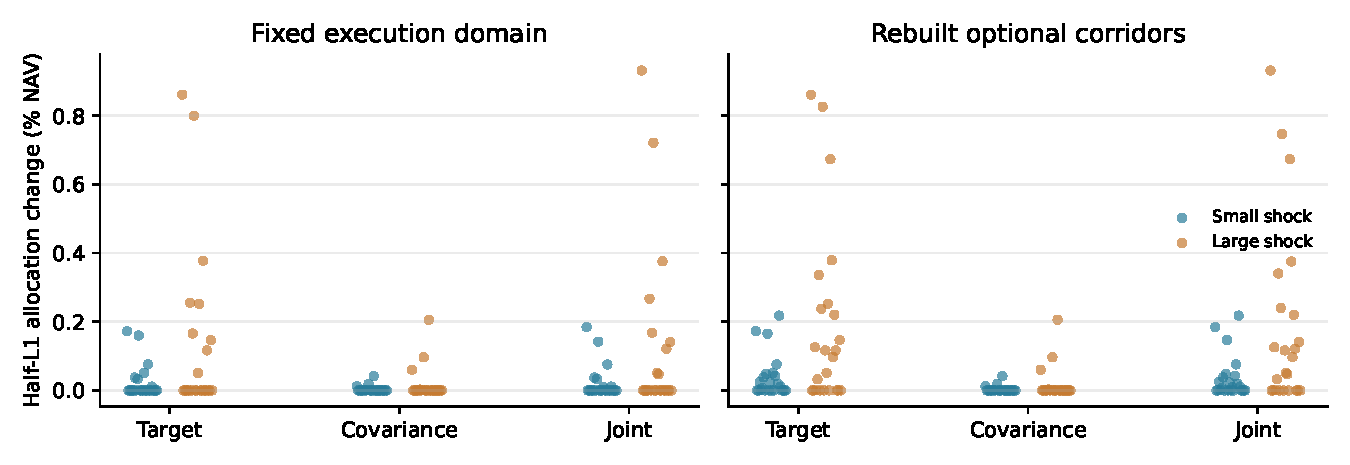
\includegraphics[width=\linewidth]{figures/sensitivity.pdf}

\caption{All conditional allocation shifts. Small/large target shocks are 10/50 NAV bp; volatility shocks have maximum absolute log shifts of 1/5 percent.}\end{figure}

\section{Full joint mixed-integer benchmark}\label{sec:joint}
\label{sec:breadth}
A frozen public synthetic grid crosses 24/72/144 nominal optional instruments, 2/6 discretionary tickets, disjoint/overlapping groups and tight/wide cash and group bands. Seed 111001 supplies 24 paired instances; seed 112001 supplies two eight-instrument controls. The generator retains two forced exits, a 50 NAV bp minimum ticket and a 25 NAV bp holding floor. The V2 heuristic and rules remain frozen. This paired rerun corrects the MIQP reference's native feasibility setting and quadratic-cone scaling after this grid exposed a false optimal termination. It is a numerical regression comparison, not an untouched validation of the corrected reference. Factorial variants share random draws and are not independent market replications.

Each joint MIQP optimises all admissible states and sizes simultaneously in the same prepared CORRIDOR domain. MIP-B starts from the common prepared incumbent; MIP-V receives only V2's audited proposal. Suffixes denote 10/60/600-second wrapper allowances. Every call starts afresh: incumbents never pass between budgets. Native calls use one thread, seed zero and the same $10^{-4}$ relative-gap setting; native integer feasibility is $10^{-9}$. Budget and start orders alternate deterministically. The mathematical MIQP is solved in an algebraically equivalent, balanced conic representation.

All 24 broad cases were attempted; 24 prepared. Effective optional candidates range from 20 to 41. Table~\ref{tab:joint} reports audited outputs over the full expected denominator. Tracking-error means use audited outputs; time summaries include every attempted arm. End-to-end (E2E) adds preparation to every arm and V2 generation to each MIP-V call.

\begin{table}[htbp]\centering\small\setlength{\tabcolsep}{4pt}
\caption{Full joint optimisation versus V2. TE is annual bp; E2E time is seconds.}\label{tab:joint}
\begin{tabular}{lrrrrr}\toprule
Arm & Audited & Mean TE & Median E2E & 95th pct. & V2 worse\\\midrule
V2 & 24/24 & 132.960 & 1.559 & 6.849 & --\\
MIP-B10 & 24/24 & 132.960 & 0.171 & 0.551 & 0\\
MIP-V10 & 24/24 & 132.960 & 1.892 & 7.202 & 0\\
MIP-B60 & 24/24 & 132.960 & 0.166 & 0.551 & 0\\
MIP-V60 & 24/24 & 132.960 & 1.895 & 7.184 & 0\\
MIP-B600 & 24/24 & 132.960 & 0.165 & 0.555 & 0\\
MIP-V600 & 24/24 & 132.960 & 1.889 & 7.219 & 0\\
\bottomrule\end{tabular}\end{table}

\begin{figure}[htbp]\centering
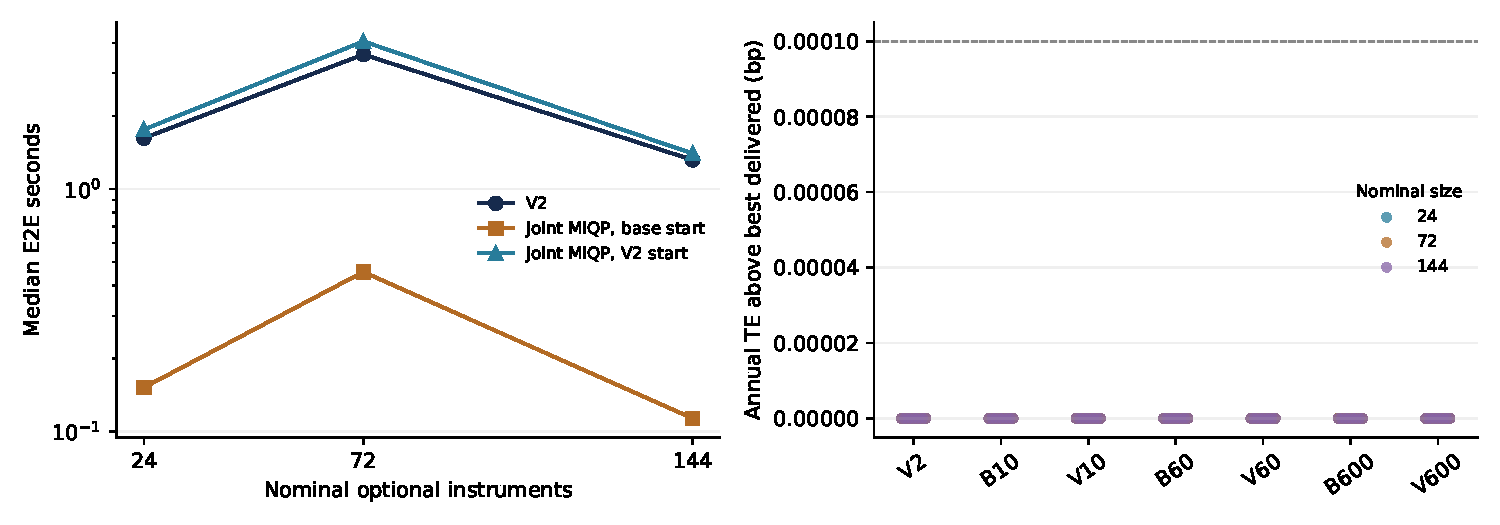
\includegraphics[width=\linewidth]{figures/joint_comparison.pdf}
\caption{Left: median E2E computation at the 600-second wrapper allowance, including preparation and V2 start generation. Right: each audited outcome above the best delivered TE on that case; this pooled reporting reference is never supplied as a start. Points identify nominal optional-universe size; the dashed line is the unchanged descriptive equality band.}\label{fig:joint}
\end{figure}

V2 exceeds the best audited delivery by more than the $10^{-4}$ bp descriptive band on 0/24 cases; its largest delivered gap is 0.000000 bp. A worse time-limited MIP delivery does not imply a worse mathematical optimum. A tie with MIP-V may simply retain V2's supplied incumbent. All native/retained/refined sources, first native audited feasibility times, failed outputs and allowance overruns are preserved in the numerical summary.

Changing the allowance changes delivered TE above the descriptive band on 0 common-base and 0 V2-started cases. These allowances are upper limits, not enforced run durations. At 600 seconds, V2 has lower TE than the common-base delivery on 0/24 cases and ties on 24/24; its largest advantage is 0.000000 bp. MIP-V600 retains the supplied V2 start on 12 cases.

Across all six MIQP arms, 0 native bounds exceed a better audited cross-arm objective at the unchanged $10^{-12}$ variance comparison scale. Raw bounds and statuses are retained, not clipped to the incumbent. Consistency with delivered witnesses is necessary but does not independently certify the native branch-and-bound result.

Separate conservative relaxation bounds close within the descriptive band on 0/24 cases. Their median/maximum best-delivery gaps are 4.153/20.025 bp; there are 0 upper/lower inconsistencies. Native optimal status and solver-reported MIP gaps remain diagnostics, not independent global certificates.

Independent full-weight QP enumeration covers 74 supports across 2 tiny cases; 2 enumerations are complete and 0 supports remain unresolved. The maximum absolute delivered difference across all tiny arms is 3.55e-09 bp. These are floating-point numerical references, not exact-arithmetic proofs.

The earlier development, holdout and search-ablation records remain in the replication package. This rerun changes only the reference's internal numerical setting, conic scaling and diagnostic checks, preserving the heuristic and production policy. Computational cost is measured rather than assumed: the experiment establishes neither a universal speed advantage nor realised investment performance.


\section{Limitations and conclusion}
Ranked Execution separates cash-funded prioritisation from the joint sizing
needed for coupled constraints. Executable states encode minimum trades and
holding alternatives; mandatory declarations make counting and exemptions
explicit. Coordinated search broadens the combinations considered under a
fixed domain, and original-unit audits control delivery.

A better objective than a time-limited mixed-integer call is not a global
certificate. An Exact improvement identifies a search or numerical limit that must
remain visible. Retained starts, native discoveries and numerical
refinements are different sources of delivered portfolios.

The empirical limits include the retrospective universe, supplied rather
than refitted estimates, dependent monthly cases and the number of genuinely
optional states after preparation. A large nominal universe does not by
itself establish difficult sparse search. The retained candidate counts
measure the scale actually tested.
Numerical corrections were informed by these instances; the sample is not
an untouched validation cohort.

This benchmark does not simulate every algorithm's recursively evolving
holdings. Such a study requires asset returns and a separate implementation
convention; its outcomes combine local decisions with path dependence.
No realised return, Sharpe ratio or trading-cost advantage follows from the
conditional comparison.

The earlier synthetic studies informed search corrections and remain in the
replication archive. The paired rerun preserves V2 and its acceptance rules;
the corrected reference was informed by these cases. The grid has 20--41
effective optional candidates, despite nominal sizes up to 144. V2 ties all
24 independent joint-MIQP deliveries within the descriptive band at every
allowance. The previously reported 3.645 bp advantage disappears. Independent
MIQP has lower median E2E cost (0.165 versus 1.559 seconds at the 600-second
allowance). Heuristic-started
MIQP matches V2 but must also pay its generation cost. None of these calls
uses the full allowance; longer allowances provide no measured improvement.

The corrected ETF and synthetic comparisons have no native bound contradicting
an audited cross-arm witness by more than $10^{-12}$ variance. Raw bounds remain
visible; this consistency check is not an independent optimality certificate.
Conservative relaxation bounds remain valid but do not close the broader
cases. The tiny enumerations agree with all arms within the descriptive band.
Together these controls support neither universal dominance nor a heuristic
speed advantage, and they do not certify global optimality on the larger cases.

The controlled sensitivity study also shows that changing input estimates and
changing the execution domain are distinct effects. All studies remain conditional
on supplied inputs and finite search budgets. External validation, broader lifecycle
changes, rolling own-book simulations and matched established alternatives remain
needed. Further algorithm changes would require fresh qualification; the present
results do not authorize a production change.
The contribution is an auditable execution heuristic with explicit
controls and reproducible evidence of both improvements and limits.

\section*{Data and code availability}
The accompanying package contains de-identified numerical decision inputs,
checksums, the ETF and synthetic runners, independent audits, reference enumeration
and table-generation code.
The reusable solver is in
\href{https://github.com/ArturSepp/OptimalPortfolios}{OptimalPortfolios}.
Tracking-error reporting uses
\href{https://github.com/ArturSepp/QuantInvestStrats}{QIS}.
This public-facing draft is prepared for release; a persistent dataset
identifier and public release URL have not yet been assigned. Execution
conditional on supplied estimates is reproduced; upstream allocation-model
estimation and raw market-data histories are outside the release.

\section*{Author declarations}
Affiliation, competing-interest and final authorship statements require
author completion before submission. AI assistance was used in implementation,
analysis and drafting; the author must review and approve the final disclosure.

\begin{thebibliography}{9}
\bibitem[Bertsimas and Cory-Wright(2022)]{bertsimas2022}
Bertsimas, D., Cory-Wright, R., 2022. A scalable algorithm for sparse portfolio
selection. INFORMS Journal on Computing 34(3), 1489--1511.
\href{https://doi.org/10.1287/ijoc.2021.1127}{doi:10.1287/ijoc.2021.1127}.
\bibitem[Guastaroba and Speranza(2012)]{kernel2012}
Guastaroba, G., Speranza, M.G., 2012. Kernel Search: An application to the
index tracking problem. European Journal of Operational Research 217(1), 54--68.
\href{https://doi.org/10.1016/j.ejor.2011.09.004}{doi:10.1016/j.ejor.2011.09.004}.
\bibitem[Mutunge and Haugland(2018)]{mutunge2018}
Mutunge, P., Haugland, D., 2018. Minimizing the tracking error of cardinality
constrained portfolios. Computers \& Operations Research 90, 33--41.
\href{https://doi.org/10.1016/j.cor.2017.09.002}{doi:10.1016/j.cor.2017.09.002}.
\bibitem[Strub and Baumann(2018)]{strub2018}
Strub, O., Baumann, P., 2018. Optimal construction and rebalancing of
index-tracking portfolios. European Journal of Operational Research 264(1), 370--387.
\href{https://doi.org/10.1016/j.ejor.2017.06.055}{doi:10.1016/j.ejor.2017.06.055}.
\end{thebibliography}
\end{document}
